% Created 2023-11-10 Fri 22:54
% Intended LaTeX compiler: pdflatex
\documentclass[11pt]{article}
\usepackage[utf8]{inputenc}
\usepackage[T1]{fontenc}
\usepackage{graphicx}
\usepackage{longtable}
\usepackage{wrapfig}
\usepackage{rotating}
\usepackage[normalem]{ulem}
\usepackage{amsmath}
\usepackage{amssymb}
\usepackage{capt-of}
\usepackage{hyperref}
\author{Agustín Alejandro Mota Hinojosa}
\date{\today}
\title{PL/SQL 4-3: Iterative Control: Basic Loops}
\hypersetup{
 pdfauthor={Agustín Alejandro Mota Hinojosa},
 pdftitle={PL/SQL 4-3: Iterative Control: Basic Loops},
 pdfkeywords={},
 pdfsubject={},
 pdfcreator={Emacs 29.1 (Org mode 9.7)}, 
 pdflang={English}}
\begin{document}

\maketitle
\tableofcontents

\section{Vocabulary}
\label{sec:org46d57c8}

Encloses a sequence of statements between the keywords LOOP and END LOOP and must execute at least once.

\textbf{Basic Loop}

Statement to terminate a loop.

\textbf{EXIT}
\section{Try it / Solve it}
\label{sec:orge175479}

\begin{enumerate}
\item What purpose does a loop serve in PL/SQL?

The purpose of loops in PL/SQL is to repeat the same or similar code a specified number of times or until a certain condition is met.

\item List the types of loops in PL/SQL.

\begin{itemize}
\item Basic Loop
\item FOR Loop
\item WHILE Loop
\end{itemize}

\item What statement is used to explicitly end a loop?

The EXIT statement is used to explicitly end a loop. It can be used alone or with a condition (EXIT WHEN condition).

\item Write a PL/SQL block to display the country\textsubscript{id} and country\textsubscript{name} values from the COUNTRIES table for country\textsubscript{id} whose values range from 1 through 3. Use a basic loop. Increment a variable from 1 through 3. Use an IF statement to test your variable and EXIT the loop after you have displayed the first 3 countries.
\begin{verbatim}
DECLARE
 v_counter NUMBER(1) := 1;
 v_country_name wf_countries.country_name%TYPE;
BEGIN
 LOOP
  SELECT country_name INTO v_country_name
  FROM wf_countries
  WHERE country_id = v_counter;
  DBMS_OUTPUT.PUT_LINE(v_country_name);
  v_counter := v_counter + 1;
  IF v_counter > 3 THEN EXIT;
  END IF;
 END LOOP;
END;
\end{verbatim}

\item Modify your solution to question 4 above, replacing the IF statement with an EXIT\ldots{}.WHEN statement.
\begin{verbatim}
DECLARE
 v_counter NUMBER(1) := 1;
 v_country_name wf_countries.country_name%TYPE;
BEGIN
 LOOP
  SELECT country_name INTO v_country_name
  FROM wf_countries
  WHERE country_id = v_counter;
  DBMS_OUTPUT.PUT_LINE(v_country_name);
  v_counter := v_counter + 1;
  EXIT WHEN v_counter > 3;
 END LOOP;
END;
\end{verbatim}

\item Create a MESSAGES table and insert several rows into it.
\begin{verbatim}
DROP TABLE messages;
CREATE TABLE messages (results NUMBER(2));
\end{verbatim}

\begin{verbatim}
DECLARE
 v_counter NUMBER(2) := 1;
BEGIN
 LOOP
  IF v_counter <> 6 AND v_counter <> 8 THEN
  INSERT INTO messages
  VALUES (v_counter);
  END IF;
  v_counter := v_counter + 1;
  EXIT WHEN v_counter > 10;
 END LOOP;
END;
\end{verbatim}
\end{enumerate}

\begin{center}
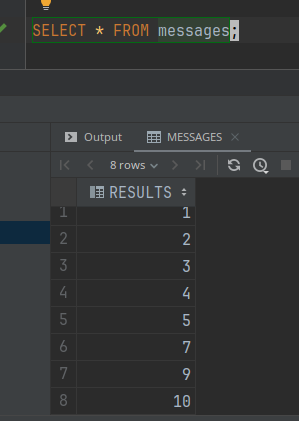
\includegraphics[width=.9\linewidth]{./resources/sall_messages.png}
\end{center}
\end{document}